
\section{Implementación}
En este capítulo expondremos la tecnología usada tanto en el servidor como en la aplicación móvil. También se comentarán las pruebas realizadas.


\subsection{Herramientas de soporte}
En esta sección explicaremos los entornos en los que se trabajo a la hora de desarrollar este proyecto, comentando los fundamento usados en ellos. Esta sección tiene una gran importancia ya que escogerlos bien al inicio nos ayudará a ganar agilidad a la hora de avanzar y cometer menos errores.


\subsubsection{• Eclipse Java EE IDE for Web Developers Version Neon2 }
Herramienta para desarrolladores  integrado (IDE)  en Java para el desarrollo de software. Fue creado por IBM como sucesor de uno de sus herramientas y ahora esta en manos de la Fundación Eclipse que es quien se encarga de seguir desarrollandolo.
 Esta herramienta de desarrollo es totalmente gratuita por lo que no encarece el precio del proyecto. Se decidió usar esta herramienta por el parecido que tiene con el entorno de Android.
\begin{figure}[H]
		\centering
		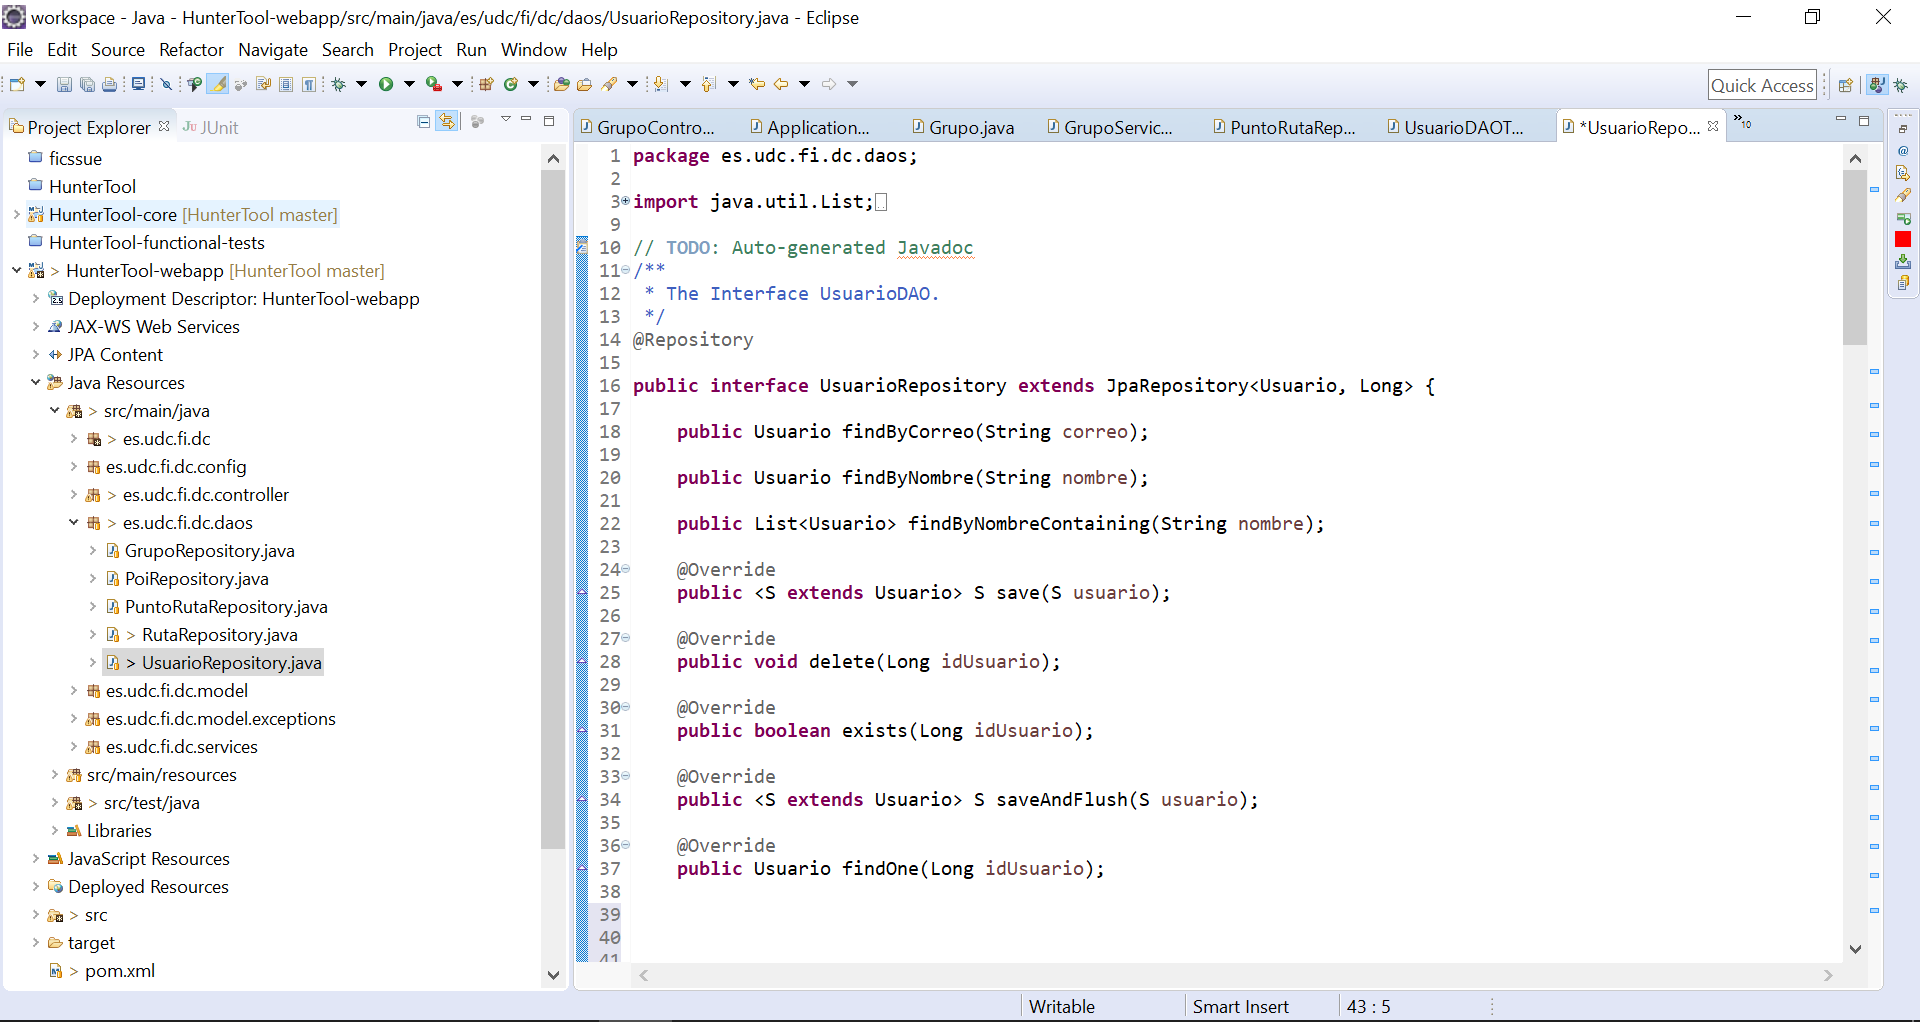
\includegraphics[width=1\textwidth] {eclipse.png}
		\caption{Entorno de trabajo Eclipse }
	\end{figure}
\subsubsection{• Spring}
Spring es un framework de código abierto que tiene como objetivo ayudar al desarrollador a trabajar con otras APIs de manera más sencilla. Nos proporciona un modelo de programación y configuración integral para aplicaciones empresariales basadas en Java, en cualquier tipo de plataforma de implementación. Simplemente es necesario añadir una dependencia, si se usa Eclipse, en el archivo pom.xml. 

\begin{figure}[H]
		\centering
		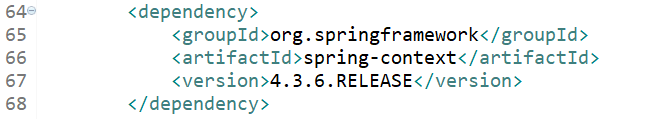
\includegraphics[width=1\textwidth] {spring.png}
		\caption{Dependencia de Spring en el pom.xml }
	\end{figure}
	
	
Como funcionalidades principales que nos ofrece y por ello elegí, serían:

\begin{itemize}
\item \textbf{Programación orientada aspectos},paradigma que nos ayuda a eliminar dependencias entre módulos acortando las lineas de código de los servicios para así poder centrarnos en la lógica de la aplicación. Lo que conlleva a reducir  la probabilidad de errores en la codificación o ineficiencias.


\item\textbf{ Inyección de dependencias}, patrón que ayuda a reducir el acoplamiento entre los distintos componentes de la aplicación. Esto lo consigue haciendo que una clase le proporcione a otra sus dependencias haciendo que la otra no tenga que crearlas ella misma. De este modo atreves de un interfaz una clase tienes las dependencias de otra sin tener que preocuparse de la implementacion de las mismas, lo que es favorable para reducir el acoplamiento.

\begin{figure}[H]
		\centering
		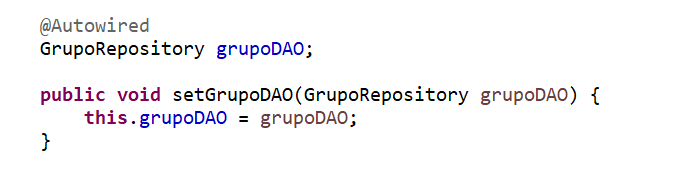
\includegraphics[width=1\textwidth] {dao.png}
		\caption{Ejemplo de inyección de dependencia }
	\end{figure}


\end{itemize}
\subsubsection{• Android Studio}
\subsubsection{• Git}
Git es un sofware para ayudarnos con el control de versiones  pensado para el mantenimiento de múltiples versiones de aplicaciones cuando estas tienen un número muy alto de archivos y queremos poder volver a un punto anterior o como copias de seguridad. A su vez Git ofrece 2 opciones para el control de versiones una mediante un interfaz y otra mediante linea de comandos.
\subsubsection{• Apache Maven}
Maven es una herramienta de software para la gestión y construcción de proyectos Java.
 Maven utiliza un Project Object Model (POM) en formato
XML para describir sus dependencias con otros módulos como jpa, firebase o postgrest. Viene con objetivos predefinidos para la compilación del código o su empaquetado.




\subsubsection{• JPA/Hibernate}
\subsubsection{• PostgreSQL}

PostgreSQL es un gestor de bases de datos objecto-relacional  que permite trabajar con grandes cargas de datos consiguiendo una tolerancia alta a errores.
Se decidió usar este gestor porqué tiene una gran adaptabilidad a otros entornos de trabajo lo que ayuda a ganar agilidad y eficiencia. También nos proporciona  el PgAdmin que facilita la gestión y administración de bases de datos ya sea mediante instrucciones SQL o con ayuda de un entorno gráfico. Permite acceder a todas las funcionalidades de la base de datos, consulta, manipulación y gestión de datos.
\subsubsection{• JUnit}

JUnit es el framework de testing para Java más extendido.
Permite la ejecución de clases Java para evaluar el comportamiento de los métodos a testar.



\subsection{Servidor}
\subsubsection{• Engadir funcionalidades a medida nos repositorios de Spring Data}
\subsection{Aplicación móvil Android}
\subsubsection{• Mapas}
\subsubsection{•}
\subsubsection{•}
\subsubsection{•}
\section{Pruebas}
\subsection{Pruebas de unidad}
\subsection{Pruebas de unidad y de integración}


